\documentclass[12pt]{report}
%\usepackage[francais]{babel}
\usepackage{lmodern}
\usepackage[a4paper]{geometry}
\usepackage[T1]{fontenc}
\usepackage[utf8]{inputenc}  
\usepackage{moreverb}
\usepackage{amsmath}
\usepackage{amsfonts}
\usepackage{amssymb}
\usepackage{textcomp}
\usepackage{pifont}
\usepackage{geometry}
\usepackage[pdftex]{graphicx}
\usepackage{graphics}
\usepackage{url}
\usepackage{graphicx}
\usepackage{float}
\usepackage{color}
\usepackage[nottoc, notlof, notlot]{tocbibind}
\usepackage[french]{varioref}
\usepackage[Glenn]{fncychap}
\usepackage{pdfpages}

\usepackage{multicol}

% entête et pied de page
%% \usepackage{fancyhdr} 
%% \pagestyle{fancy}
%% \renewcommand{\chaptermark}[1]{\markboth{#1}{}}
%% \renewcommand{\sectionmark}[1]{\markright{\thesection\ #1}}
%% \fancyhf{} \fancyhead[LE,RO]{\bfseries\thepage}
%% \fancyhead[LO]{\bfseries\rightmark}
%% \fancyhead[RE]{\bfseries\leftmark}
%% \renewcommand{\headrulewidth}{0.5pt}
%% \addtolength{\headheight}{0.5pt}
%% \renewcommand{\footrulewidth}{0pt}
%% \fancypagestyle{plain}{ \fancyhead{}
%% \renewcommand{\headrulewidth}{0pt}} 

% pour inclure du code par exemple
\usepackage{listings}

\lstset{%configuration de listings
float=hbp,%
basicstyle=\ttfamily\small, %
columns=flexible, %
tabsize=2, %
frame=trBL, %
frameround=tttt, %
extendedchars=true, %
showspaces=false, %
showstringspaces=false, %
numbers=left, %
numberstyle=\tiny, %
breaklines=true, %
breakautoindent=true, %
captionpos=b,%
xrightmargin=0cm, %
xleftmargin=-0cm, %
language=tex, %
frameround=fttt;%
}

%%%%%%%%%%%%%%%% Lengths %%%%%%%%%%%%%%%%
\geometry{a4paper,twoside,left=2cm,right=2cm,marginparwidth=1.2cm,marginparsep=3mm,top=1.7cm,bottom=1.5cm}

\newcommand{\stamp}{{\tt \textit{Stamp }}}
\newcommand{\class}{{\tt \textit{class }}}
\newcommand{\initarg}{{\tt \textit{Initarg }}}
\bibliographystyle{plain}
\urlstyle{sf}

%%%%%%%%%%%%%%%%%%%%%%%%%%%%%%%%%%%%%%%%%%%%%%%

\newenvironment{vcenterpage}
{\newpage\vspace*{\fill}}
{\vspace*{\fill}\par\pagebreak}

\newtheorem{ex}{Exemple}%[section]
\newtheorem{theo}{Theorem}
\newcommand{\tuple}[1]{\ensuremath{\langle #1 \rangle}}

\begin{document}
%%%% Page de titre %%%%
% =============== 
% set of variables 
% ===============

% the title
\def\presentation{PER PROJECT DEFENCE}
\def\bottomTitle{PER PROJECT}
\def\noteAboutAuthor{Engeneering students/ENSEIRB-MATMECA}
\def\subject{Grid deformation for data visualization}
%\def\subject{Déformation de Grille pour la visualisation d'information}
% =================
% Header
% =================
\title[\bottomTitle]{
        {\bfseries \huge \presentation\\} 
        {\bfseries \subject}\\
        {\small\bf A. Lambert, R. Bourqui, D. Auber}\\   
}

\titlegraphic{
  
\includegraphics[scale=0.15]{../rapport/img/logobordeaux1.jpg}
  \hspace{2cm}
  
\includegraphics[scale=0.25]{../rapport/img/noms.png}
  \hspace{2cm}
  
\includegraphics[scale=0.25]{../rapport/img/logo.jpg}
}

\author[\noteAboutAuthor]{
  {\normalsize \bfseries \sffamily Clients : }
  David {\sc Auber} \hspace{1cm} Romain {\sc Bourqui}\\    
}



%%%% remerciement %%%%%%%
% \chapter*{Thanks}

% \addcontentsline{toc}{chapter}{Thanks}

%%%%% terminologie %%%%%%%%%%
%% \newpage

\def\termea{\bf \footnotesize xx}
\def\sensa{\footnotesize xx}

\def\termeb{\bf \footnotesize xx}
\def\sensb{\footnotesize xx}

\def\termec{\bf \footnotesize xx}
\def\sensc{\footnotesize xx}

\def\termed{\bf \footnotesize }
\def\sensd{\footnotesize }

\def\termee{\bf \footnotesize }
\def\sense{\footnotesize }

\def\termef{\bf \footnotesize }
\def\sensf{\footnotesize }

\def\termeg{\bf \footnotesize }
\def\sensg{\footnotesize }

\def\termeh{\bf \footnotesize }
\def\sensh{\footnotesize }

\def\termei{\bf \footnotesize }
\def\sensi{\footnotesize }

\def\termej{\bf \footnotesize }
\def\sensj{\footnotesize }

\def\termek{\bf \footnotesize }
\def\sensk{\footnotesize }



\begin{center}
\subsubsection*{Terminologie}
\begin{tabular}{|p{5cm}|p{12cm}|}
\hline
{\bf ~~~~~ T{\scriptsize ERME}} &  {\bf ~~~~~~~~~~~~~~~~~~~ S{\scriptsize IGNIFICATION}}\\
\hline
\hline
\termea & \sensa\\
\hline
\termeb & \sensb\\
\hline
\termec & \sensc\\
\hline
\termed & \sensd\\
\hline
\termee & \sense\\
\hline
\termef & \sensf\\
\hline
\termeg & \sensg\\
\hline
\termeh & \sensh\\
\hline
\termei & \sensi\\
\hline
\termej & \sensj\\
\hline
\termek & \sensk\\
\hline

\end{tabular}
 
\end{center}


%%%% resume %%%%%%%%%
\begin{abstract}
  The article we are currently working on deals with how to visualize graphs containing many nodes and edges. With huge amount of data generally comes visual clutter, in our case due to edges crossing. This solution is based on an edge bundling technique coupled with a grid built from the original graph. Authors also used a GPU-based rendering method to highlight bundles densities without losing edge color. We use in our solution the Tutte algorithm in order to quickly obtain a graph without crossing, based on a triangular-face grid, which helps to read relationship between nodes. This algorithm will be available as a Tulip plugin. 

\end{abstract}

%%%% plan %%%%%
\tableofcontents
%\listoffigures
%\listoftables



%%%%% corps du rapport %%%%%%%%%
\chapter*{Introduction}

The article summarized in this document was written by A.Lambert, R.Bourqui and D . Auber, researchers in LaBRI in Bordeaux.


This article speaks about how to visualize graphs containing many nodes and edges. With improvements in data acquisition comes an increase of the size and the complexity of graphs and this huge amount of data generally causes visual clutter, in our case due to edges crossing.
For example, it could be interesting to visualize data in fields like biology, social sciences, data mining or computer science and then emphasize their high-level pattern to help users perceive underlying models.


Nowadays, in the research world, the information is easily represented into graphs to visualize more and more data. However, this huge amount of information prevents the graph from being manually drawn:  It explains the need of software able to generate an appropriate graph with all nodes and edges. Yet this graph may suffer from cluttering, which should be reduced for a better understanding.


The first part of this document presents review related work on reducing edge clutters and enhancing edge bundles visualization, with which the article is connected. The second will deal with the Tutte algorithm , followed by the implementation issues. A third part will show our results. Finally, we draw a conclusion and explain the limits of our work for further improvements.

\addcontentsline{toc}{chapter}{Introduction}


\chapter{The context}

\frame{
  \frametitle{The context}
\begin{center} 
Easy understanding with effective representation
 \end{center}
  \begin{figure}[H]
    \centering
    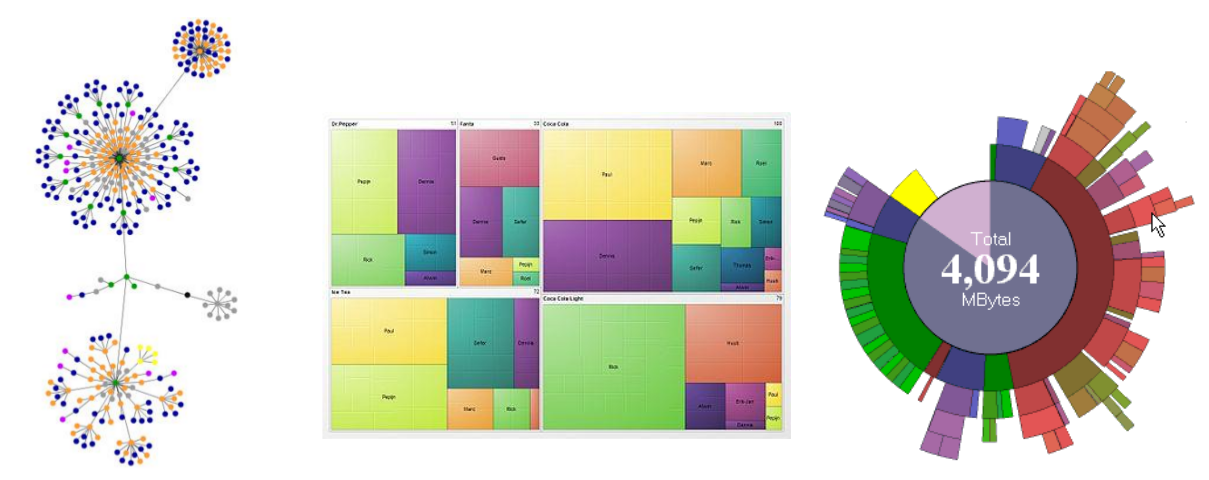
\includegraphics[scale=0.29]{../rapport/img/graphes_jolis.png}
  \end{figure}
  \pause
  \begin{alertblock}{}
    Only available for few graphs
\end{alertblock}
\vspace{1cm}
} 

\frame{
  \frametitle{The context}
  \framesubtitle{Two different methods}
  \begin{figure}[H]
    \centering
    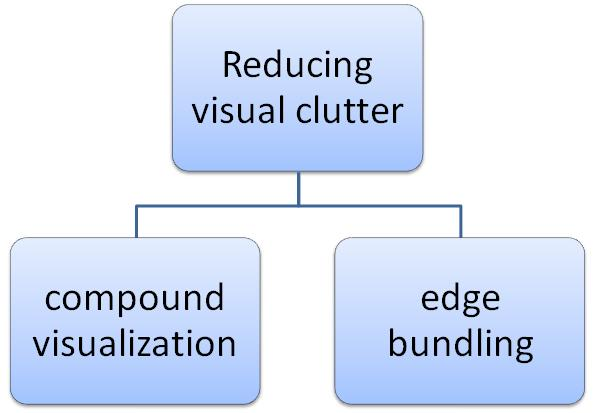
\includegraphics[scale=0.4]{../rapport/img/slide3.jpg}
  \end{figure}
 
\vspace{1cm}
} 

\frame{
  \frametitle{The context}
  \framesubtitle{Compound visualization}
  \begin{figure}[H]
    \centering
    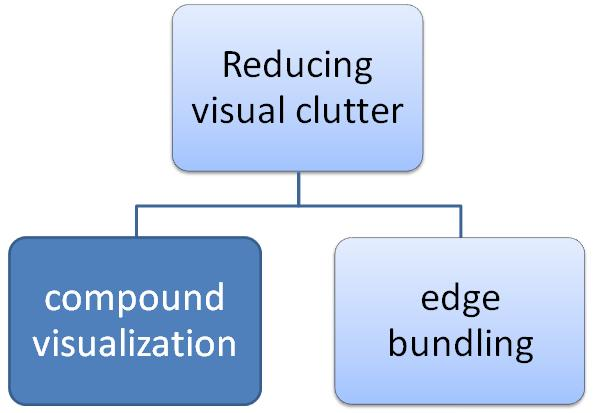
\includegraphics[scale=0.4]{../rapport/img/slide4.jpg}
  \end{figure}
 
\vspace{1cm}
} 

\frame{
  \frametitle{The context}
  \framesubtitle{Compound visualization}
  
  \begin{columns}[!ht]
    \begin{column}{4cm}
    \begin{block}{}   
     \begin{itemize}
     \item Nodes gathered into metanodes\\
     \item Inter-cluster edges merged into metaedges
     \end{itemize}
     \end{block}
    \end{column}
    \begin{column}{6cm}   
      \begin{figure}[H]
        \centering
        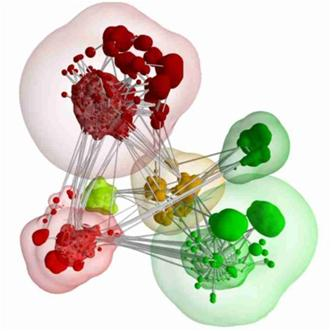
\includegraphics[scale=0.5]{../rapport/img/slide5.jpg}
      \end{figure}
    \end{column}
  \end{columns}
 \pause

  \begin{alertblock}{}
  \centering
    Impossibility for some nodes to move:
    node positions bring information
\end{alertblock}

\vspace{1cm}
} 

\frame{
  \frametitle{The context}
  \framesubtitle{Edge bundling}
  \begin{figure}[H]
    \centering
    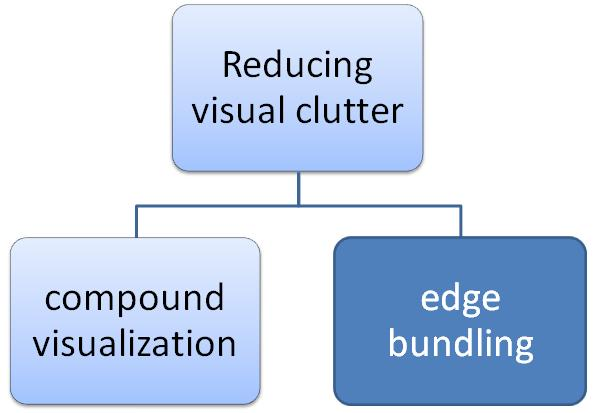
\includegraphics[scale=0.4]{../rapport/img/slide6.jpg}
  \end{figure}
 
\vspace{1cm}
} 

\frame{
  \frametitle{The context}
  \framesubtitle{Edge bundling}

\begin{alertblock}{}
  \centering
    Impossibility for some nodes to move:
    node positions bring information
\end{alertblock}
\pause
\begin{figure}[H]
        \centering
        
\includegraphics[scale=0.2]{../rapport/img/fleche.png}
      \end{figure}
\begin{center}
\begin{exampleblock}{}
\centering
Keep node position but edge aggregation
\end{exampleblock}
\end{center}                 
\pause 
 \begin{columns}[!ht]
\vspace{1cm}
    \begin{column}{6cm} 
    \begin{block}{}
    \centering
    Routes edges into bundles
    \end{block}
    \end{column}
    \begin{column}{6cm}   
      \begin{figure}[H]
        \centering
        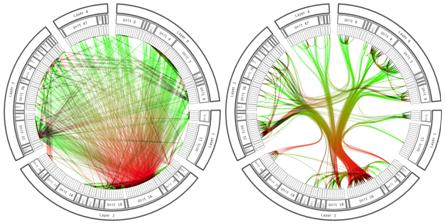
\includegraphics[scale=0.5]{../rapport/img/slide7_2.jpg}
      \end{figure}
    \end{column}
  \end{columns}

} 


%\chapter{Previous works}

\chapter{Tutte}

\section{Tutte's algorithm}

This part of text comes from the article~\cite{pa}.

In this paper, we will use basic graph theory terminology, see for
example~\cite{pb}. Let $G=(V,E)$ be a planar graph. A mapping $\Gamma$
of $G$ into the plane is a function $\Gamma : V \cup E \to P(\mathbb{R}^2)$
which maps a vertex $v \in V$ to a point in $\mathbb{R}^2$ and an edge $e =
uv \in E$ to the straight line segment joining $\Gamma(u)$ and
$\Gamma(v)$.  A mapping is an embedding if distinct vertices are mapped to
distinct points, and the open segment of each edge does not intersect any
other open segment of an edge or a vertex.

In 1963, Tutte~\cite{pc} gave a way to build embeddings of any planar,
3-connected graph $G=~(V,E)$. Let $C$ be a cycle whose vertices are the
vertices of a face of G in some (not necessarily straight-line) embedding
of $G$. Let $\Gamma$ be a mapping of $G$ into the plane, satisfying the
conditions:

\begin{itemize}

\item the set Ve of the vertices of the cycle C is mapped to the vertices of a strictly
convex polygon Q, in such a way that the order of the points is respected;

\item each vertex in $V_i = V \ V_e$ is a barycenter with positive coefficients of
its adjacent vertices (Tutte assumed all coefficients to be equal to 1, but
the proof extends without changes to this case). In other words, the images
v of the vertices v under $\Gamma$ are obtained by solving a linear system
(S): for each $u \in V_{i, v|uv \in E} \lambda_{uv} (u - v) = 0$, where the
$\lambda_{uv}$ are positive reals. It can be shown that the system (S) admits
a unique solution.

\end{itemize}

\begin{theo} \label{theo:box}
(Tutte’s Theorem) $\Gamma$ is an embedding of G into the plane, with
strictly convex interior faces.
\end{theo}


% \begin{thebibliography}{99}

% \bibitem{pa} E. Colin de Verdière, M. Pocchiola, and G. Vegter. Tutte's Barycenter Method applied to Isotopies. \emph{Computational Geometry: Theory and Applications, 26}, 81–97, 2003.

% \bibitem{pb} B. Bollob's. Modern graph theory, \emph{volume 184 of Graduate Texts in Mathematics}. Springer-Verlag, 1998.

% \bibitem{pc} W. T. Tutte. How to draw a graph. \emph{Proceedings of the London Mathematical Society}, 13:743–768, 1963.

% \end{thebibliography}




\section{Tutte Sequential}

To obtain the graph resulted of the Tutte's theorem, an algorithm is
needed. In this section, a sequential algorithm is described. This
algorithm is an iterative solution. To compute a solution, a set of node
that constitute a convex polygon must be decided. Let $P$ this set of node. Let
$G_k$ be the graph generated at the step $k$.
\\

To obtain the graph of the next step, all the node of the interior of the
convex polygon $P$ will be visited. For each node visited, the barycentric
coordinates of its neighbourhood is computed. Then this coordinates is used
to update the position of the current node. Once each node were visited,
the computation of the graph $G_{k+1}$ is finished.
\\
In this project, the stop condition used for this algorithm is an epsilon
between the relative positions of the node of the graph $G_k$ and
$G_{k+1}$. For all node of the graph, if the length of each movement is
inferior to a given epsilon, the graph $G_{k+1}$ is the solution.
\\

Following is a synthetic view of this algorithm : 
\begin{verbatim}
G = {V,E}
P = set of node constitute a convex polygon
procedure tutte(G, P, epsilon)
  epsilon_current = 0
  for each node of (V \ convex polygon)
    barycenter = barycenter of node
    epsilon_current = max(epsilon_current, distance(node, barycenter)
    node = barycenter
  if (epsilon_current < epsilon)
    exit()
  tutte(G, P, epsilon)
\end{verbatim}


% Le but ici est d'exposé la méthode algorithmique qui découle de l'algorithme de Tutte et  de prouver que cette méthode converge (retrouver l'article qui en parle)


\section{Tutte Parallel Algorithms}
%here should be the implementation of Tutte with basic structure 

%\subsection{Sequentiel version}
%in this first optimization Frozar you are suggested to put the improvement due to the new data structure you took

\subsection{Asynchronous parallel version}
%in this optimization Frozar you are suggested to talk about results with openMP

\subsubsection{Distribution of nodes: Graph coloring}
In order to implement a parallel asynchronous version of Tutte algorithm, it is necessary to separate graph nodes into different sets. The objectif is to extract an independance between nodes. In fact, each node have to move while maintaining neighbors positions. Thus, the independance must be between node and his neighbors. This problem is similar to the famous problem of graph colorating.
\paragraph*{}
The objectif of the modified Tutte algorithm is to handle graph of thousands nodes. To separate such a number of nodes, it is more performant to use a heuristic of the algorithm of graph coloring.\\
The greedy algorithm is a simple and good solution to separate nodes into sets fastly and effictively.
\paragraph*{}
The algorithm used in this project is :
\begin{verbatim}
G={V,E}
Y = V
color = 0
While Y is not empty
   Z = Y
   While Z is not empty
      Choose a node v from Z
      Colorate v with color
      Y = Y - v
      Z = Z - v - {neighbors of v}
   End while
   color ++
End while
\end{verbatim}
\subsubsection{Applying Tutte algorithm to sets}
Once a sets of nodes is obteined, it is possible to apply a parallel Tutte algorithm. The question is how to parallelize it on sets of nodes. The natural idea is to attribute one sets per thread :
\begin{figure}[!h]
\centering
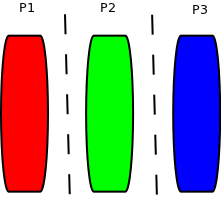
\includegraphics[scale=0.5]{img/distribution_verticale.png}
\caption{One set per thread}
\end{figure}
This distribution is far from being optimal. In fact, each thread have to lock neighbors node before moving it, wich introduce an importante critical section. In addition to being unfair, this distribution is limited by number of sets produced.\\

The best distribution for sets obteined by graph coloring is to execute $n$ threads on one set. Each thread move an number of nodes of the set without any critical section. This is because each node of the set is not the neighbor of all others nodes of the same set. Once the thread finish moving all his nodes of the set, he must wait for others threads (implemented by a barrier). After, the same processus is applyed on the next set.

\begin{figure}[!h]
\centering
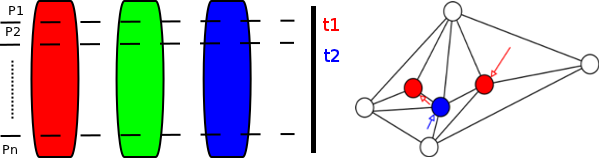
\includegraphics[scale=0.5]{img/distrib.png}
\caption{$n$ threads per set}
\end{figure}


Reference : Introduction to Algorithms (Cormen, Leiserson, Rivest, and Stein) 2001, Chapter 16 "Greedy Algorithms".


\subsection{Synchronous parallel version}
%in this optimization Ozenati you are suggested to talk about the asynchronous implementation (if faster than the others) with graph coloration



\chapter{Implementations}

\section{Graph representation for Tulip}

%it is asked here to talk about the situation of the graph is before we start the implementation: how do we manage to have the graph

%It is asked here to talk briefly about the algorithm we are going to use in the project: how it works (hope you see what I mean) 


\section{Data Structure}
%here sould be presented the first data structure used
In the implementation of our sulution we have defined our own data structure on which we excute the Tutte's algorithm. We have implemented some mechanisms to convert a tulip format graph to our own graph structure and also to get informations from our structure inserted in a tulip format graph. In other words our structure is a temporary structure for storing informations about nodes in order to execute the Tutte's algorithm.

\subsection{Aim}
As a format tulip contains a lot of informations so it costs a lot to manipulate them and so far away we do not need all the informations about a given tulip graph. To point out we especially do not need all the properties about nodes to conduct the Tutte's algorithm.For intance, for a given node we just want to know if it is fixed for a fixed node's position nevers changes during the tutte's algorithme. In addition of that, as we are looking for performance, we need a light and adapted structure to the principe of Tutte's algorithm. Below are some of criterias which make us thought we need a new data structure.
\begin{enumerate}
\item The fact that a given node is fixed or not is indicated firsly by a mobility property. However there is anover property incating nodes wich are part of graph contouring and these nodes need to be fixed too. So to deal with the fact that a given node is fixed or not we need to manipulate two properties that cost a lot.

\item In tulip format there is an hierarchy of graphs or we only need
  the parent of the graph, the one which is not subgraph of another
  one. we do not need the sub-graph relation between graphs.

\item 

\end{enumerate}  

\subsection{First implementation}
In order to avoid memory leak and implemente easily the Tutte's
algorithme, we merely stock in our sttructure only the informations
needed to run the algorithm. We implemented our structure so that one
can easily access the neighbourhood of a given node for it is very
crucial in a Tutte'algorithm. To do this we define a class that
contains diferent informations needed on a given node (the attibuts)
and all the operations we need to run on a node (the methods).

\newpage
\begin{lstlisting}
class MyNode {
 private:
  node n;
  bool mobile;
  Coord coord;  
  vector<MyNode *> voisin;

 public:
  MyNode();
  MyNode(const node n, const Coord coord);
  MyNode(const node n, const bool mob, const Coord coord);
  ~MyNode();
  
  const node getNode() const;
  bool getMobile() const;
  void setMobile(const bool b);
  const Coord getCoord() const;
  void setCoord(const Coord &);
  vector<MyNode *> * getVoisin();
  vector<MyNode *> getVoisin() const;
};
\end{lstlisting}

\subsubsection{The vertex's attributs needed}


\subsubsection{The operations on a vertex}

\subsection{Enhanced implementation}

%% \subsubsection{Distribution of nodes: Graph coloring}
In order to implement a parallel asynchronous version of Tutte algorithm, it is necessary to separate graph nodes into different sets. The objectif is to extract an independance between nodes. In fact, each node have to move while maintaining neighbors positions. Thus, the independance must be between node and his neighbors. This problem is similar to the famous problem of graph colorating.
\paragraph*{}
The objectif of the modified Tutte algorithm is to handle graph of thousands nodes. To separate such a number of nodes, it is more performant to use a heuristic of the algorithm of graph coloring.\\
The greedy algorithm is a simple and good solution to separate nodes into sets fastly and effictively.
\paragraph*{}
The algorithm used in this project is :
\begin{verbatim}
G={V,E}
Y = V
color = 0
While Y is not empty
   Z = Y
   While Z is not empty
      Choose a node v from Z
      Colorate v with color
      Y = Y - v
      Z = Z - v - {neighbors of v}
   End while
   color ++
End while
\end{verbatim}
\subsubsection{Applying Tutte algorithm to sets}
Once a sets of nodes is obteined, it is possible to apply a parallel Tutte algorithm. The question is how to parallelize it on sets of nodes. The natural idea is to attribute one sets per thread :
\begin{figure}[!h]
\centering
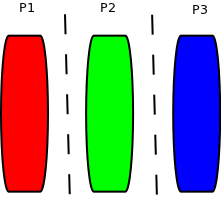
\includegraphics[scale=0.5]{img/distribution_verticale.png}
\caption{One set per thread}
\end{figure}
This distribution is far from being optimal. In fact, each thread have to lock neighbors node before moving it, wich introduce an importante critical section. In addition to being unfair, this distribution is limited by number of sets produced.\\

The best distribution for sets obteined by graph coloring is to execute $n$ threads on one set. Each thread move an number of nodes of the set without any critical section. This is because each node of the set is not the neighbor of all others nodes of the same set. Once the thread finish moving all his nodes of the set, he must wait for others threads (implemented by a barrier). After, the same processus is applyed on the next set.

\begin{figure}[!h]
\centering
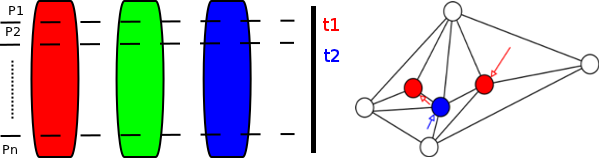
\includegraphics[scale=0.5]{img/distrib.png}
\caption{$n$ threads per set}
\end{figure}


Reference : Introduction to Algorithms (Cormen, Leiserson, Rivest, and Stein) 2001, Chapter 16 "Greedy Algorithms".


\section{Results}
\subsection{Benchmark}

The authors provided us with three graphs in order to test our
different implementations of the Tutte method.\\

These graphs have the following characteristics :

\begin{center}
\begin{tabular}{|c|c|c|}
\hline
Graph & number of vertices & number of edges \\
\hline
aiir\_traffic & 14693 & 63403\\
imdb & 9488 & 33942\\
migration & 14318 & 49460\\
\hline
\end{tabular}
\end{center}


For the first implementation with a basic structure to
work on the graph, we obtain these results~:

\begin{center}
\begin{tabular}{|c|c|c|c|}
\hline
Graph & number of iterations & mean time of execution of Tutte's algorithm & standard deviation\\
\hline
aiir\_traffic & 61 & 0.2526 & 0\\
imdb & 473 & 1.2957 & 0\\
migration & 5 & 0.006314 & 0\\
\hline

\end{tabular}
%\caption{title}
\end{center}

\subsection{Not planar graph}
The results we get here are not as good as we expected. Although the
computation time is quite improved, the produced graphs are not planar. The
reason is that the provided graph has some fixed nodes inside the
grid. Consequently, after the call of our implementation of the Tutte
Algorithm, some edges crossing (due to those fixed nodes) appear and remove
the planarity of the graph.

As an explanation, we can say that moving nodes tend to be oriented to the 
side which has the highest level of fixed nodes.(see the figure \ref{mauvais_1}). 
With such a graph, a mobile node which is opposite to the side with numerous
edges will move to this side and create an edge-crossing (see the figure \ref{mauvais_2}).

\begin{figure}[!h]
  \begin{minipage}[!h]{.5\linewidth}
   \centering
   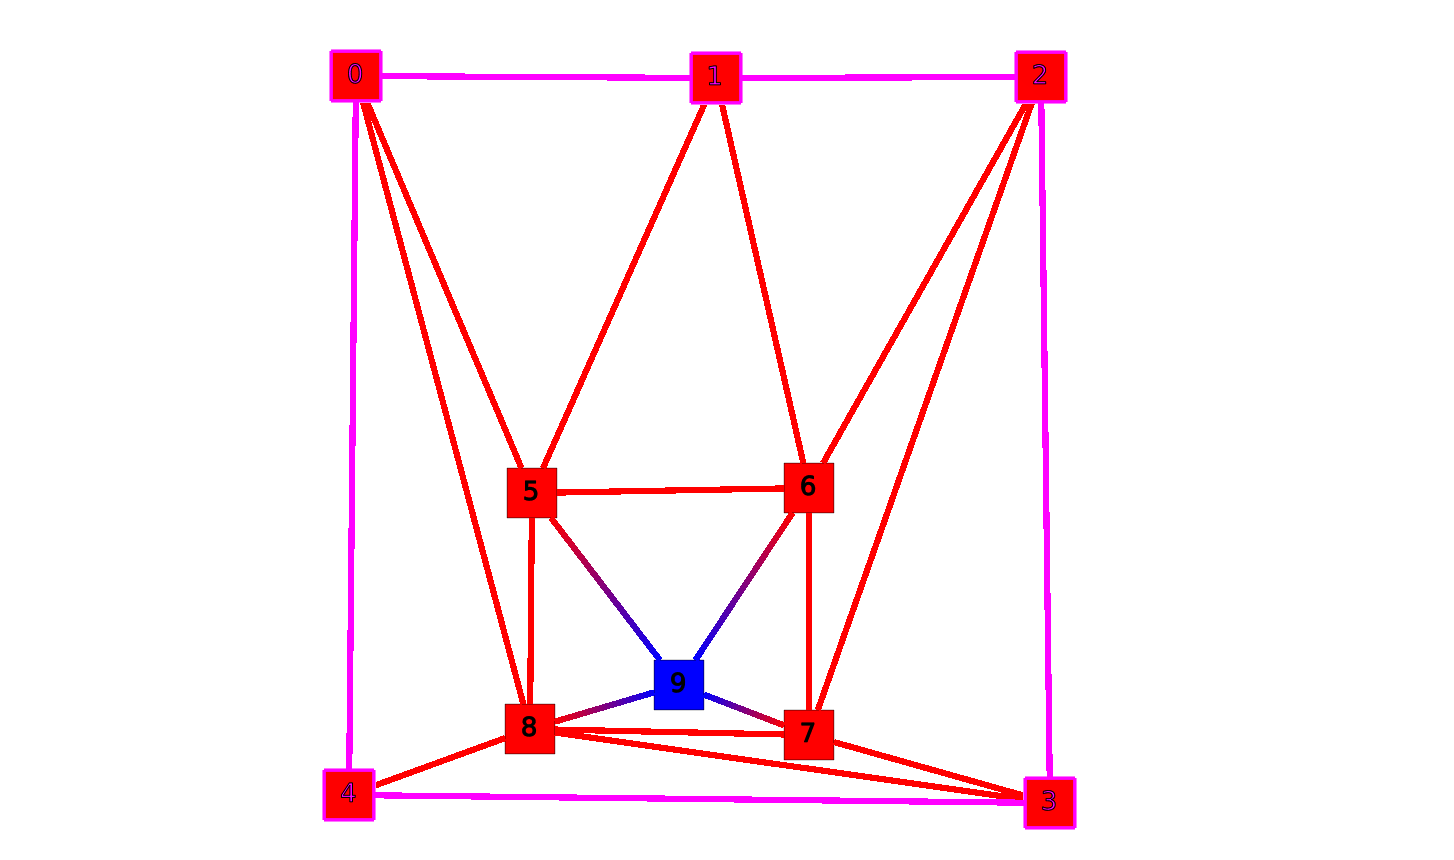
\includegraphics[scale=0.27]{snapshots/constate_fix_init.png}
   \caption{The initial graph. The blue node is fixed}
   \label{mauvais_1}
 \end{minipage} \hfill
 \begin{minipage}[!h]{.45\linewidth}
   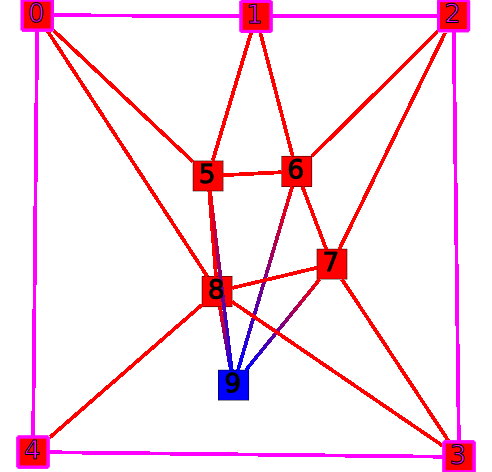
\includegraphics[scale=0.45]{snapshots/constate_probleme.png}
   \caption{The set not correctly modified}
   \label{mauvais_2}
 \end{minipage}
\end{figure}

%\newpage 

You can notice that if all the nodes in the interior of boundaries are mobile, then the graph produced stay planar (see figure \ref{correct_1} and \ref{correct_2}).

\begin{figure}[!h]
  \begin{minipage}[!h]{.5\linewidth}
    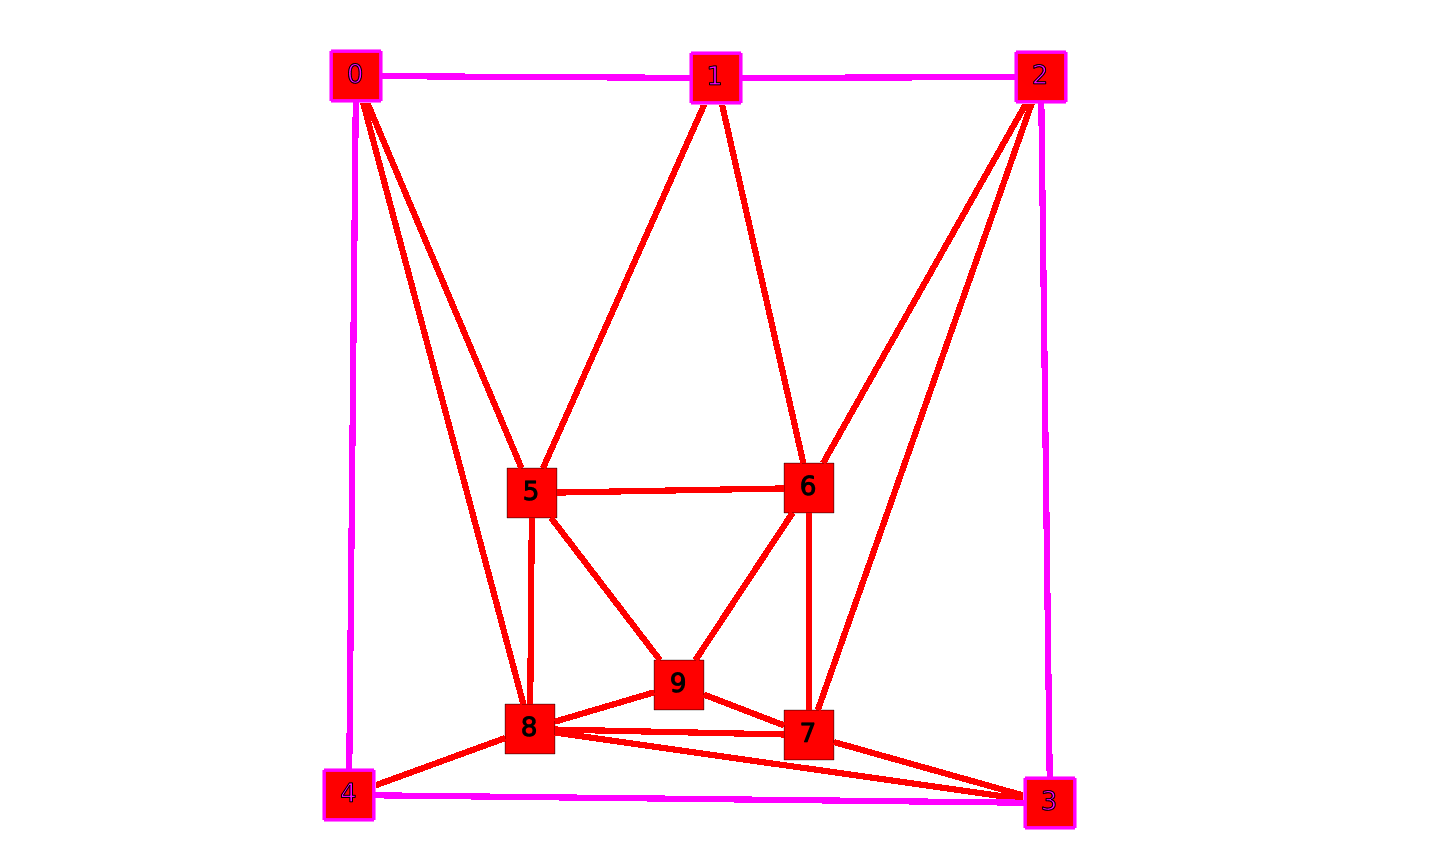
\includegraphics[scale=0.27]{snapshots/constate_mobil_init.png}
    \caption{The initial graph with all interior nodes mobile}
    \label{correct_1}
  \end{minipage}
  \begin{minipage}[!h]{.55\linewidth}
    \centering
    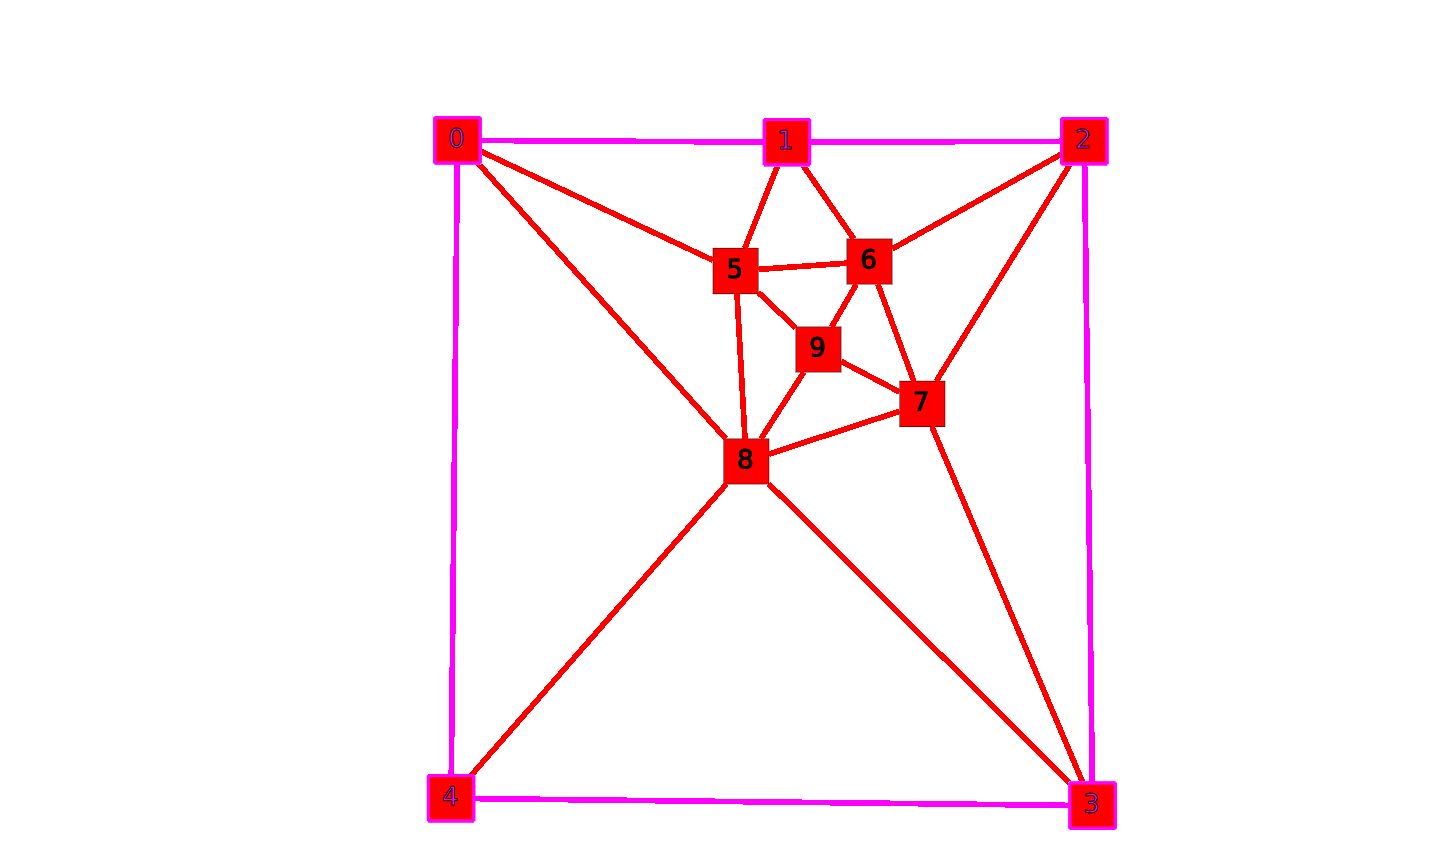
\includegraphics[scale=0.29]{snapshots/constate_nikel.png}
    \caption{The graph correctly modified}
    \label{correct_2}
  \end{minipage} \hfill
\end{figure}


\addcontentsline{toc}{chapter}{Conclusion}
\chapter*{Conclusion}


With our best Tutte algorithm implementation , we obtain an algorithm convergence in 5 iterations and it spends x seconds to recalculate all the coordinates. (à mettre à jour)
Finally, our optimizations allowed an improvement of the clutter reduction and the performance compared with existent methods.


After discussing with our teachers in charge, some issues concerning our standalone version remains unresolved and could be taken into account in the future: Rather than working with input graph nodes, it would be interesting to dynamically add nodes (and their edges to keep a triangular-face graph) and launch again the algorithm in order to refine given results. It will also be quite interesting to automatically join small triangles or divide big triangles into littles ones. 

(à rajouter: plugin, prouver que ca marche: peut etre dû à la construction de la grille (triangulation de delaunay + contrainte: deux sommets fixes ne sont jamais reliés par une arête sauf sur le contour))

%I suggest here to talk about what can be do in the future (there is a quite start of this in my context written in Wiki) 
\begin{thebibliography}{}

\bibitem{pa} E. Colin de Verdière, M. Pocchiola, and G. Vegter. Tutte's Barycenter Method applied to Isotopies. \emph{Computational Geometry: Theory and Applications, 26}, 81–97, 2003.

\bibitem{pb} B. Bollob's. Modern graph theory, \emph{volume 184 of Graduate Texts in Mathematics}. Springer-Verlag, 1998.

\bibitem{pc} William T. Tutte. How to draw a graph. \emph{Proceedings of the London Mathematical Society}, 13:743–768, 1963.

\bibitem{pd} A. Lambert, R. Bourqui, and D. Auber. Winding roads: Routing edges
into bundles. \emph{In 12th Eurographics/IEEE-VGTC Symposium on
Visualization (Computer Graphics Forum; Proceedings of EuroVis
2009).} To appear., 2010.

\bibitem{pe} A. Lambert, R. Bourqui, and D. Auber. 3D edge bundling for
geographical data visualization. \emph{In IV ’10: Proceedings of the 14
International Conference on Information Visualisation (IV’09)},
Washington, DC, USA, 2010. IEEE Computer Society.

\bibitem{pf} Gormen, T.H. and Leiserson, C.E. and Rivest, R.L. and Stein, C. Introduction to algorithms. \emph{In MIT press Cambridge, MA}, 16:"Greedy Algorithms", 1990.

\textbf{(refaire biblio en se centrant plus sur tutte)}


% \bibitem{1} 

% \bibitem{2} 

% \bibitem{3} 

% \bibitem{4} 

% \bibitem{5} 
   
\end{thebibliography}


%%%%%% Liste des annexes %%%%%%%%%%
%% \part{Annexes}
%% \appendix
%% \chapter{the appendix's name}

\end{document}
